\chapter{Исследовательская часть}

\section{Интерфейс приложения}

На рисункaх  \ref{fig:interface} -- \ref{fig:working} приведено изображение интерфейса главного экрана приложения.

\begin{figure}[h!]
	\centering{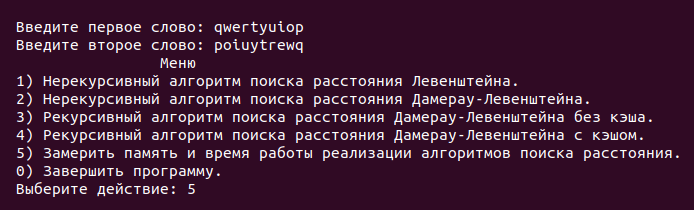
\includegraphics[scale=0.7]{photos/interface.png}}
	\caption{Интерфейс}
	\label{fig:interface}
\end{figure}


На экране приложения пользователь может ввести два слова, для которых необходимо вычислить расстояние, а также выбрать метод, который будет использован для этого вычисления. 
В результате выводится полученное расстояние, память и скорость работы алгоритмов, показывающие, как время выполнения операций (измеряемое в секундах) зависит от количества выполненных операций.

\begin{figure}[h!]
	\centering{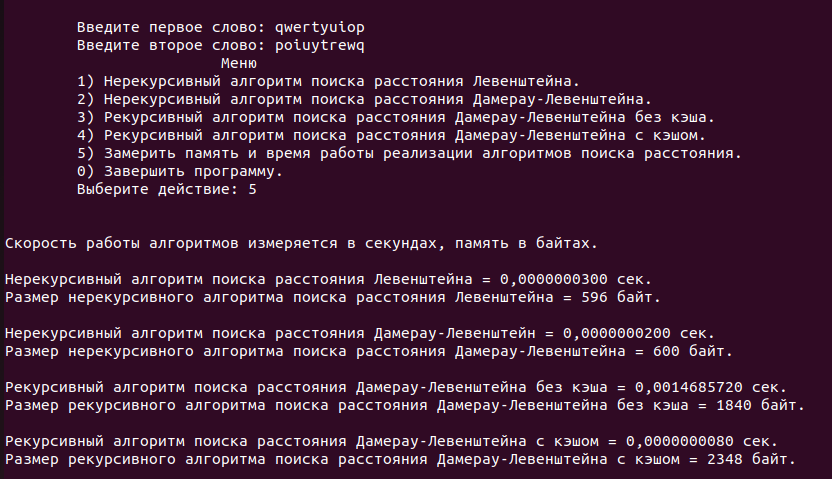
\includegraphics[scale=0.4]{photos/working.png}}
	\caption{Экран с результатом}
	\label{fig:working}
\end{figure}

\clearpage

\section{Технические характеристики}

Технические характеристики устройства, на котором выполнялось тестирование:

\begin{itemize}
	\item операционная система -- Ubuntu 22.04.3 LTS;
	\item оперативная память -- 12 Гб;
	\item процессор -- AMD® Athlon silver 3050u with radeon graphics × 2;
\end{itemize}

\section{Время выполнения реализаций алгоритмов}

На рисунке 4.3 приведено сравнение реализации всех алгоритмов поиска расстояния, у которых строки длиной от 1 до 10.
\begin{figure}[ht!]
	\begin{center}
		\captionsetup{singlelinecheck = false, justification=centerfirst}
		\begin{tikzpicture}
			\begin{axis}[
				xlabel={Длина слова},
				ylabel={Время в секундах},
				width = 0.95\textwidth,
				height=0.8\textheight,
				xmin=0, xmax=10,
				ymode=log, 
				legend pos=north west,
				legend style={font=\footnotesize},
				xmajorgrids=true,
				grid style=dashed,
				]
				
				\addplot[
				blue,
				semithick,
				mark = *,
				mark size = 3pt,
				thick,
				] file {graph/leven.csv};
				
				\addplot[
				red,
				semithick,
				mark = *,
				] file {graph/dam_leven.csv};
				
				\addplot[
				green,
				semithick,
				mark = *,
				] file {graph/recursive.csv};
				
				\addplot[
				purple,
				semithick,
				mark = *,
				] file {graph/cache_recursive.csv};
				
				\legend{
					Нерекурсивный алгоритм поиска расстояния Левенштейна,
					Нерекурсивный алгоритм поиска расстояния Дамерау -- Левенштейна,
					Рекурсивный алгоритм поиска расстояния Дамерау -- Левенштейна без кэша,
					Рекурсивный алгоритм поиска расстояния Дамерау -- Левенштейна с кэшом
				}
			\end{axis}
			
		\end{tikzpicture}
		\centering
		\caption{Сравнение времени работы реализаций алгоритмов}
		\label{fig:graph1}
	\end{center}
	
\end{figure}

\clearpage

\section{Используемая память}

Введены следующие обозначения:
\begin{itemize}
	\item$n$ --- длина строки $S_{1}$;
	\item$m$ --- длина строки $S_{2}$;
	\item$size()$ --- функция вычисляющая размер в байтах;
	\item $string$ --- строковый тип;
	\item $int$ --- целочисленный тип;
	\item $size\_t$ --- беззнаковый целочисленный тип.
\end{itemize}

Максимальная глубина стека вызовов при рекурсивной реализации нахождения расстояния Дамерау -- Левенштейна равна сумме входящих строк, а на каждый вызов требуется 2 дополнительные переменные, соответственно, максимальный расход памяти равен:
\begin{equation}
	\label{eq:dl_rec_memory}
	(n + m) \cdot (2 \cdot size(string) + 3 \cdot size(int) + 2 \cdot sizeof(size\_t)),
\end{equation}
где:
\begin{itemize}
	\item $2 \cdot size(string)$ --- хранение двух строк;
	\item $2 \cdot size(size\_t)$ --- хранение размеров строк;
	\item $2 \cdot size(int)$ --- дополнительные переменные;
	\item $size(int)$ --- адрес возврата.
\end{itemize}

Для рекурсивного алгоритма c кешированием поиска расстояния Дамерау -- Левенштейна будет теоретически схож с расчетом в формуле (\ref{eq:dl_rec_memory}), но также учитывается матрица, соответственно, максимальный расход памяти равен:
\begin{equation}
	\label{eq:dl_hash_memory}
	\begin{aligned}
		(n + m) \cdot (2 \cdot size(string) + 3 \cdot size(int) + 2 \cdot size(size\_t)) + \\
		+ (n + 1) \cdot (m + 1) \cdot size(int)
	\end{aligned}
\end{equation}
Использование памяти при итеративной реализации алгоритма поиска расстояния Левенштейна теоретически равно:
\begin{equation}
	\label{eq:lev_mtr_memory}
	\begin{aligned}
		(n + 1) \cdot (m + 1) \cdot size(int) + 2 \cdot size(string) + 2 \cdot size(size\_t) + \\
		+ size(vector<vector<int>>) + (n + 1) \cdot size(vecotr<int>) + 2 \cdot size(int),
	\end{aligned}
\end{equation}
где 
\begin{itemize}
	\item $2 \cdot size(string)$ --- хранение двух строк;
	\item $2 \cdot size(size\_t)$ --- хранение размеров матрицы;
	\item $(n + 1) \cdot (m + 1) \cdot size(int)$ --- хранение матрицы;
	\item $size(vector<vector<int>>) + (n + 1) \cdot size(vecotr<int>)$ --- указатель на матрицу;
	\item $size(int)$ --- дополнительная переменная для хранения результата;
	\item $size(int)$ --- адрес возврата.
\end{itemize}

Использование памяти при итеративной реализации алгоритма поиска расстояния Дамерау -- Левенштейна теоретически равно:
\begin{equation}
	\label{eq:dl_mtr_memory}
	\begin{aligned}
		(n + 1) \cdot (m + 1) \cdot size(int) + 2 \cdot size(string) + 2 \cdot size(size\_t) + \\
		+ size(vector<vector<int>>) + (n + 1) \cdot size(vecotr<int>) + 3 \cdot size(int),
	\end{aligned}
\end{equation}
где 
\begin{itemize}
	\item $2 * size(string)$ --- хранение двух строк;
	\item $2 \cdot size(size\_t)$ --- хранение размеров матрицы;
	\item $(n + 1) \cdot (m + 1) \cdot size(int)$ --- хранение матрицы;
	\item $size(vector<vector<int>>) + (n + 1) \cdot size(vecotr<int>)$ --- указатель на матрицу;
	\item $2 \cdot size(int)$ --- дополнительные переменные;
	\item $size(int)$ --- адрес возврата.
\end{itemize}

По расходу памяти итеративные алгоритмы проигрывают рекурсивным: максимальный размер используемой памяти в итеративном растет как произведение длин строк, в то время как у рекурсивного алгоритма -- как сумма длин строк.

\begin{figure}[ht!]
	\begin{center}
		\captionsetup{singlelinecheck = false, justification=centerfirst}
		\begin{tikzpicture}
			\begin{axis}[
				xlabel={Длина слова},
				ylabel={Память в байтах},
				width = 1.04\textwidth,
				height=0.9\textheight,
				xmin=0, xmax=100,
				ymode=log, 
				legend pos=north west,
				legend style={font=\footnotesize},
				xmajorgrids=true,
				grid style=dashed,
				]
				
				\addplot[
				blue,
				semithick,
				mark = *,
				mark size = 3pt,
				thick,
				] file {graph/leven_memory.csv};
				
				\addplot[
				red,
				semithick,
				mark = *,
				] file {graph/dam_leven_memory.csv};
				
				\addplot[
				green,
				semithick,
				mark = *,
				] file {graph/recursive_memory.csv};
				
				\addplot[
				purple,
				semithick,
				mark = *,
				] file {graph/cache_recursive_memory.csv};
				
				\legend{
					Нерекурсивный алгоритм поиска расстояния Левенштейна,
					Нерекурсивный алгоритм поиска расстояния Дамерау -- Левенштейна,
					Рекурсивный алгоритм поиска расстояния Дамерау -- Левенштейна без кэша,
					Рекурсивный алгоритм поиска расстояния Дамерау -- Левенштейна с кэшом
				}
			\end{axis}
			
		\end{tikzpicture}
		\centering
		\caption{Сравнение размеров реализаций алгоритмов в байтах}
		\label{fig:graph2}
	\end{center}
	
\end{figure}


Из данных, видно, что рекурсивные алгоритмы являются более эффективными по памяти, так как используется только память под локальные переменные, передаваемые аргументы и возвращаемое значение, в то время как итеративные алгоритмы затрачивают память линейно пропорционально длинам обрабатываемых строк.

Из рисунка~\ref{fig:graph2} видно, что рекурсивная реализация алгоритма поиска расстояния Дамерау - Левенштейна эффективная по памяти, чем итеративная.
\clearpage

\section*{Вывод}

В данном разделе было произведено сравнение количества затраченного времени и памяти алгоритмов поиска расстояний Левенштейна и Дамерау- Левенштейна. 
Наименее затратным по времени оказался итеративный алгоритм нахождения расстояния Левенштейна.
Рекурсивная реализация алгоритма поиска расстояния Дамерау - Левенштейна будет более затратным по времени по сравнению с итеративной реализацией алгоритмов поиска расстояния, но менее затратным по памяти.

